% Main content slides

\section{Load Balancing}

\begin{frame}{Symmetric Domain}
  \begin{figure}
    \begin{center}
      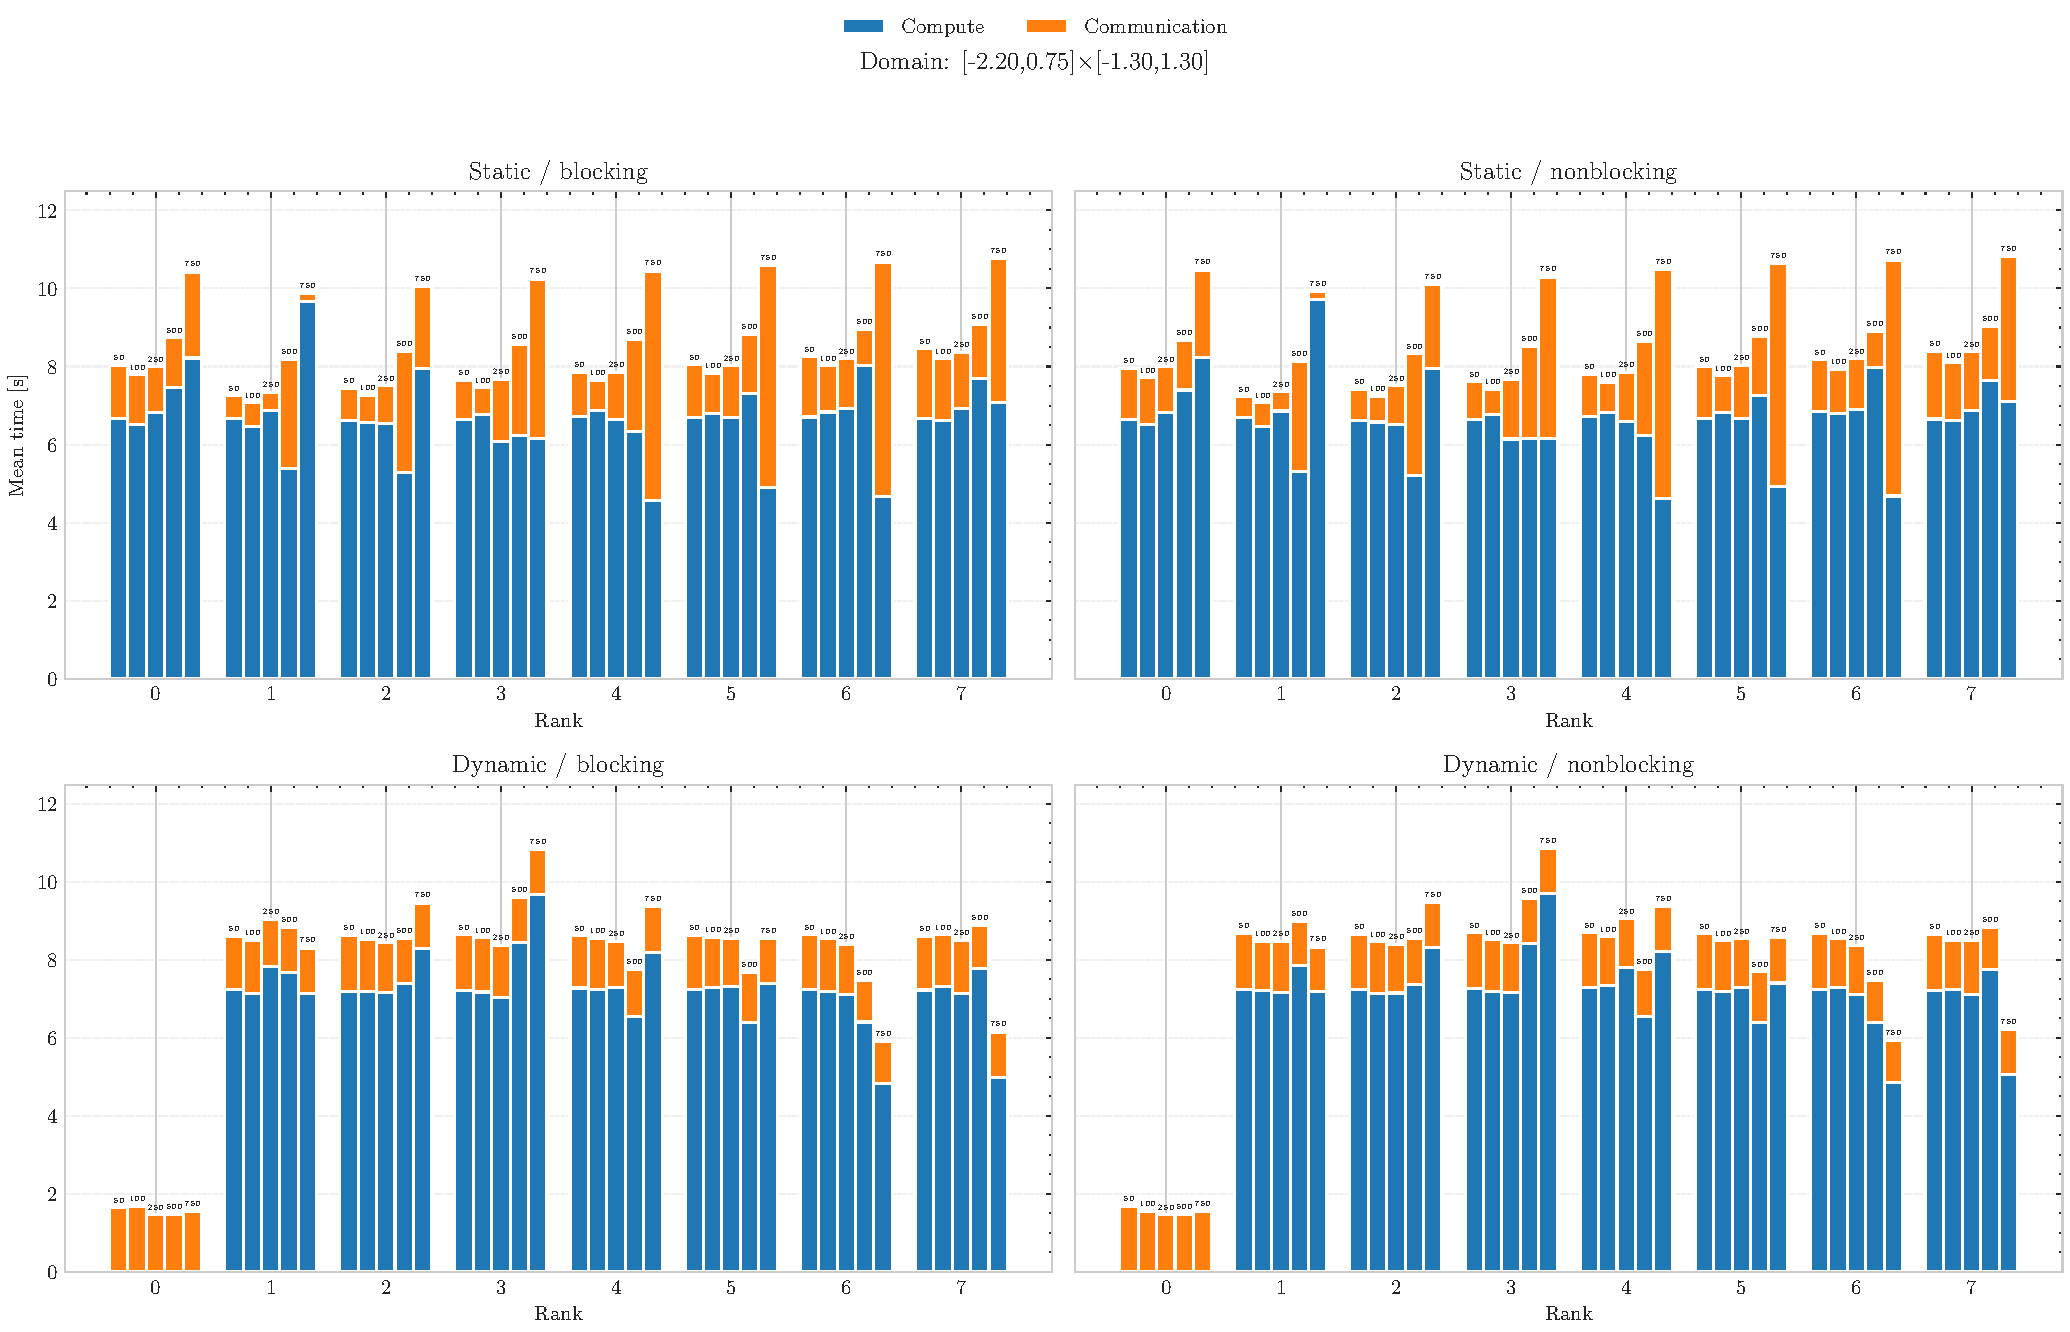
\includegraphics[width=0.75\textwidth]{figures/Plots/2_load_balancing/2.0Ranks_2_20_0_75_1_30_1_30.pdf}
    \end{center}
  \end{figure}
    
\end{frame}


\section{Scaling}\label{sec:scaling} % (fold)


% section Scaling (end)
\begin{frame}{Two Column Layout}
    \begin{columns}
        \column{0.5\textwidth}
        \begin{figure}
          \begin{center}
            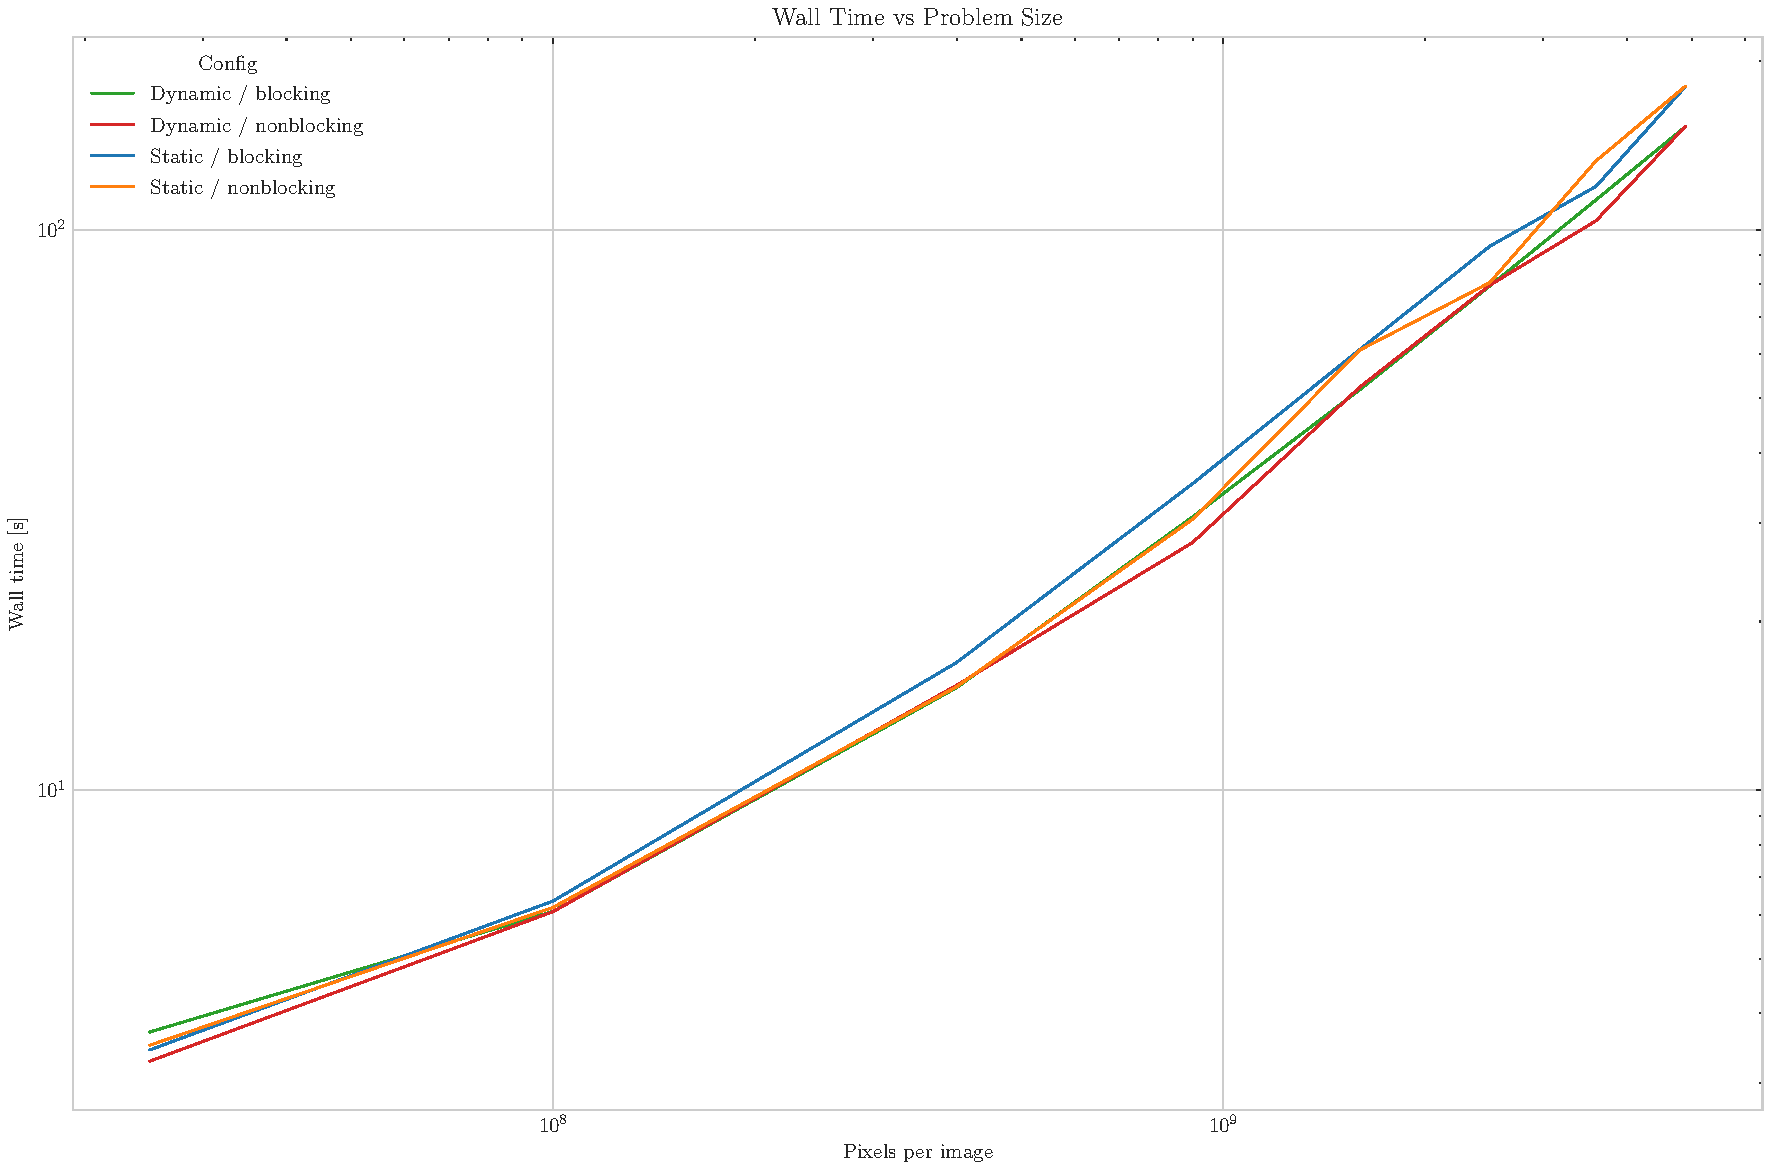
\includegraphics[width=1.15\textwidth]{figures/Plots/4_scaling_problem/4.1_wall_time_vs_pixels.pdf}
            \caption*{Scaling with problem size}\label{fig:wall_time_vs_pixels}
          \end{center}
        \end{figure}
        

        \column{0.5\textwidth}
        \begin{figure}
          \begin{center}
            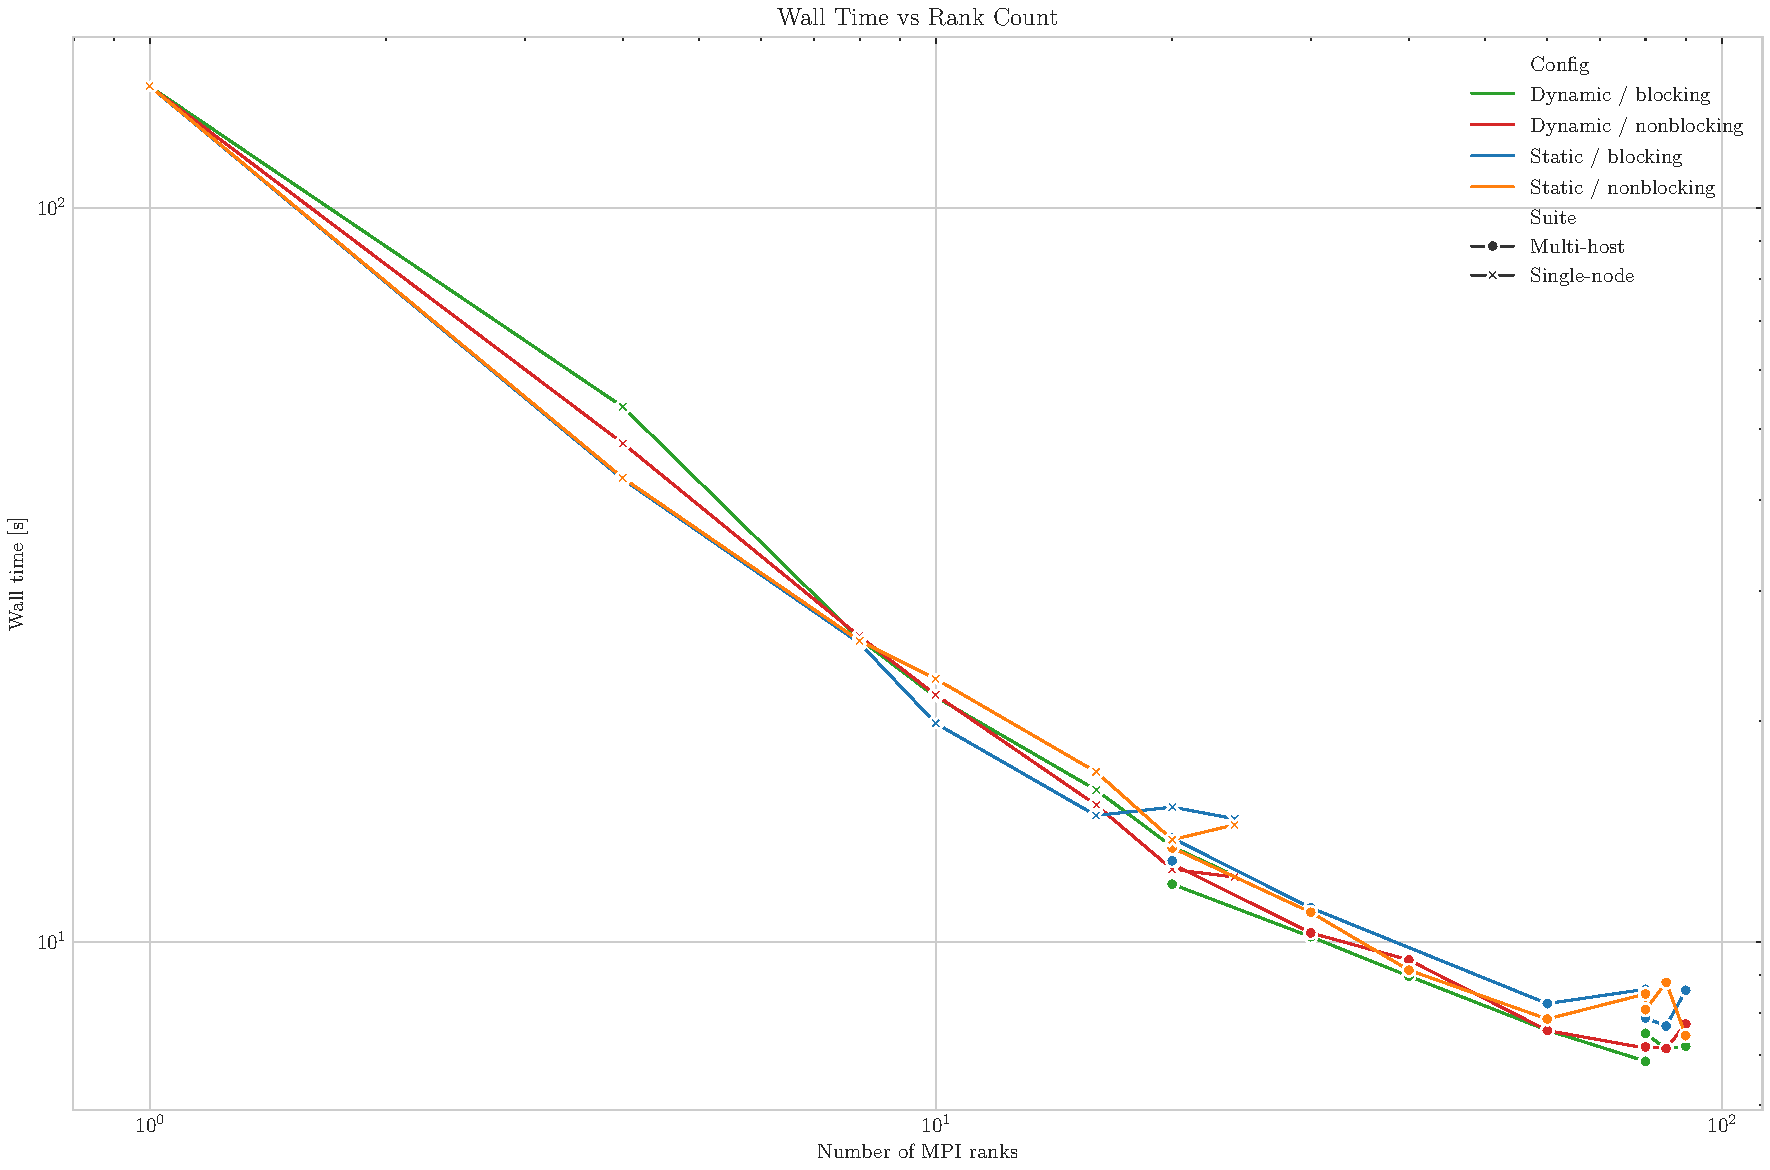
\includegraphics[width=1.15\textwidth]{figures/Plots/5_scaling_ranks/5.1_wall_time_vs_ranks.pdf}
            \caption*{Scaling with number of ranks}\label{fig:wall_time_vs_ranks}
          \end{center}
        \end{figure}
          
    \end{columns}
\end{frame}

